\newpage


% \section{Application Mobile Livreur}
% Développée en Flutter/React Native, elle comprend :
% \begin{itemize}
%     \item \textbf{Tracking GPS :} Envoi de la position en arrière-plan.
%     \item \textbf{Gestion des Missions :} Système de "Push Notifications" pour accepter/refuser une course.
%     \item \textbf{Wallet :} Visualisation du solde et déclenchement des virements vers le compte bancaire.
%     \item \textbf{Navigation :} Intégration de Google Maps / Waze pour l'itinéraire.
% \end{itemize}





cha\section{Application Mobile Livreur}
\label{sec:application_mobile}

L'application mobile est l'outil de travail exclusif du livreur. Elle doit être robuste, économe en énergie, et capable de maintenir une connexion constante avec le Backend, même dans des conditions réseau dégradées.

\subsection{Directives Techniques : La Stack Mobile}

Pour maximiser le partage de code et de compétences avec l'équipe Web, le développement s'orientera vers les technologies cross-platform, tout en utilisant des modules natifs pour les fonctionnalités critiques.

\begin{itemize}
    \item \textbf{Framework (UI \& Logique) :} \textbf{React Native (avec Expo Bare Workflow)}. Ces frameworks permettent de compiler une application native pour iOS et Android à partir d'une seule base de code.
    \item \textbf{Gestion d'État Local :} \textbf{Zustand} (pour React Native). Essentiel pour gérer l'état de la course en cours et le solde du Wallet sans ralentir l'interface.
    \item \textbf{Temps Réel \& Notifications :} \textbf{Firebase Cloud Messaging (FCM)} pour les notifications Push (réveil de l'application), couplé à \textbf{Socket.io-client} pour le flux de données continu lorsque l'application est ouverte.
    \item \textbf{Géolocalisation métier :} Utilisation de librairies natives spécialisées (ex: \texttt{react-native-background-geolocation}) pour garantir le suivi GPS même quand le téléphone est verrouillé, tout en optimisant la batterie.
\end{itemize}

\subsection{Diagramme d'États : Cycle d'Activité et Tracking GPS}

Le comportement du composant GPS et les requêtes réseau dépendent entièrement du statut du livreur. Le diagramme ci-dessous dicte aux développeurs quand activer ou désactiver l'envoi de la position pour préserver la batterie.

\begin{figure}[ht!]
    \centering
    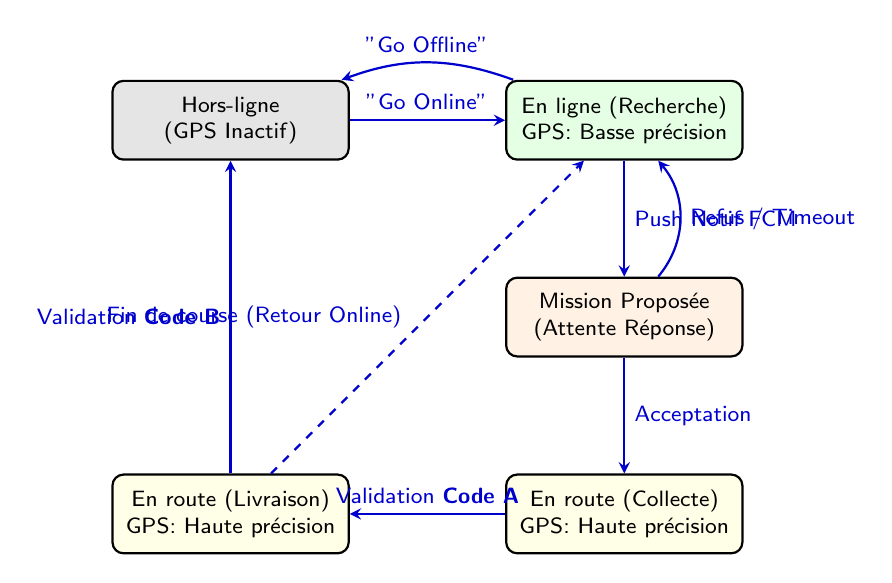
\begin{tikzpicture}[
        font=\sffamily\footnotesize,
        >=stealth,
        state/.style={draw, thick, rounded corners=4pt, fill=blue!5, minimum width=3cm, minimum height=1cm, align=center},
        action/.style={->, thick, blue!80!black}
    ]

    % Noeuds
    \node[state, fill=gray!20] (offline) at (0, 0) {Hors-ligne\\(GPS Inactif)};
    \node[state, fill=green!10] (online) at (5, 0) {En ligne (Recherche)\\GPS: Basse précision};
    \node[state, fill=orange!10] (proposed) at (5, -2.5) {Mission Proposée\\(Attente Réponse)};
    \node[state, fill=yellow!10] (collecte) at (5, -5) {En route (Collecte)\\GPS: Haute précision};
    \node[state, fill=yellow!10] (livraison) at (0, -5) {En route (Livraison)\\GPS: Haute précision};

    % Flèches
    \draw[action] (offline) -- node[above]{"Go Online"} (online);
    \draw[action] (online) edge[bend right=20] node[above]{"Go Offline"} (offline);
    
    \draw[action] (online) -- node[right]{Push Notif FCM} (proposed);
    \draw[action] (proposed) edge[bend right=40] node[right]{Refus / Timeout} (online);
    
    \draw[action] (proposed) -- node[right]{Acceptation} (collecte);
    \draw[action] (collecte) -- node[above]{Validation \textbf{Code A}} (livraison);
    
    \draw[action] (livraison) -- node[left]{Validation \textbf{Code B}} (offline);
    % Note : On le renvoie hors-ligne ou en ligne selon la logique métier, mettons vers En Ligne :
    \draw[action, dashed] (livraison) -- node[left, xshift=-0.2cm]{Fin de course (Retour Online)} (online);

    \end{tikzpicture}
    \caption{Machine à états du Livreur dictant le comportement du module GPS.}
    \label{fig:mobile_states}
\end{figure}

\subsection{Directives d'Implémentation par Fonctionnalité}

L'équipe de développement mobile devront porter une attention particulière aux points d'intégration suivants :

\subsubsection{1. Tracking GPS (L'enjeu critique)}
\begin{itemize}
    \item \textbf{Throttling et Batching :} L'application ne doit pas envoyer une requête HTTP à chaque mètre parcouru. Elle doit accumuler les points GPS locaux (SQLite/AsyncStorage) et les envoyer par lots (batch) au Backend via WebSocket toutes les 5 à 10 secondes.
    \item \textbf{Permissions OS :} Le code doit gérer rigoureusement les demandes de permissions "Localiser toujours" (iOS/Android). Sans cette permission, le système d'exploitation tuera l'application en arrière-plan.
\end{itemize}

\subsubsection{2. Gestion des Missions et Push Notifications}
\begin{itemize}
    \item \textbf{Deep Linking :} Lorsqu'une notification "Nouvelle Course" arrive, un appui sur celle-ci doit ouvrir l'application directement sur la modale de la mission (Deep Link interne).
    \item \textbf{Mécanisme de Timeout :} La proposition de course doit inclure un compte à rebours visuel (ex: 30 secondes). Si le livreur ne répond pas, l'application doit rejeter silencieusement la course pour que le Backend la réaffecte à un autre livreur (Redis Queue).
\end{itemize}

\subsubsection{3. Navigation et Itinéraires}
\begin{itemize}
    \item L'application mobile ne doit pas calculer les itinéraires elle-même. Les développeurs implémenteront des liens profonds (URI Schemes) pour déléguer la navigation aux applications natives du téléphone.
    \item \textbf{Exemple d'implémentation :} L'appui sur le bouton "Naviguer" déclenchera un \texttt{Linking.openURL('waze://?ll=lat,lng\&navigate=yes')} pour Waze, ou \texttt{google.navigation:q=lat,lng} pour Google Maps.
\end{itemize}

\subsubsection{4. Module Wallet et Virements}
\begin{itemize}
    \item \textbf{Sécurité Financière :} Le solde affiché dans l'application doit être purement consultatif (lecture seule). La demande de virement appelle un endpoint Backend strict (ex: intégré avec l'API \textbf{Stripe Connect} ou équivalent) qui vérifiera le solde réel côté serveur avant d'initier le transfert bancaire.
\end{itemize}